\documentclass[../part_2.tex]{subfiles}

\begin{document}
    \subsection{Алгоритм обучения}
    \par Для обучения было решено модернизировать алгоритм dino для работы с текстом.
    \par Для этого было необходимо сделать:
    \begin{itemize}
        \item Модифицировать репозиторий \acrshort{dino} для работы с оригинальной архитектурой трансформера
        \item Преобразовать multicrop augmentation
        \item Выбрать подходящие аугментации
    \end{itemize}
    \subsubsection{Описание архитектуры нейронной сети}
    \par Изначально в методе обучения \acrshort{dino} была использована архитектура ViT -- адаптация трансформерной архитектуры для обработки изображений, где входное изображение разбивается на последовательность неперекрывающихся патчей, которые линейно преобразуются в вектора  embedding. Для составления единого вектора представления в начало последовательности добавляют токен CLS, финальное отображение которого используют для downstream задач. 
    \par Использованная архитектура ViT в \acrshort{dino} разбивала исходное изображение на кусочки размером $16\times16$ пикселей. Затем к ним прибавлялись Positional Embeddig и эти данные передавались дальше в блоки модели.
    \begin{figure}[H]
        \centering
        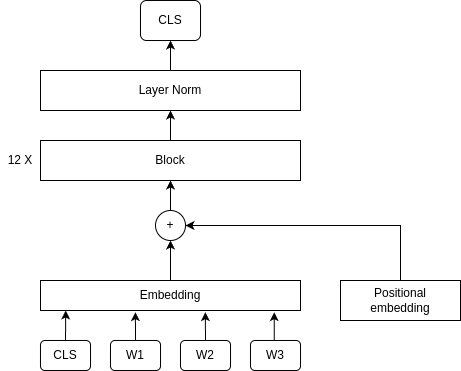
\includegraphics[width=0.6\textwidth]{model_arc.png}
        \caption{Архитектура нейросети}
        \label{fig:model_arc}
    \end{figure}
    \par Для изменения линейного преобразования был использован Embedding слой, который каждому токену присваивает свой вектор представления.
    \begin{figure}[H]
        \centering
        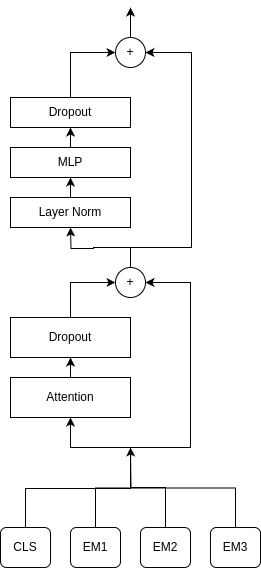
\includegraphics[height=0.6\textwidth]{nn_block.png}
        \caption{Архитектура блока нейросети}
        \label{fig:nn_block}
    \end{figure}
    \par Блок состоит из слоя нормирования, внимания, dropout, еще раз нормирования и MLP. Из них самым полезным и ресурсозатратным является слой внимания. Его вычисление зависит от квадрата числа токенов в последовательности.
    \par Так как изначальное изображение было размером $224\times224$, то в Vit модели было всего 196 токенов. В текстовой же реализации токенов значительно больше.
    \begin{figure}[H]
        \centering
        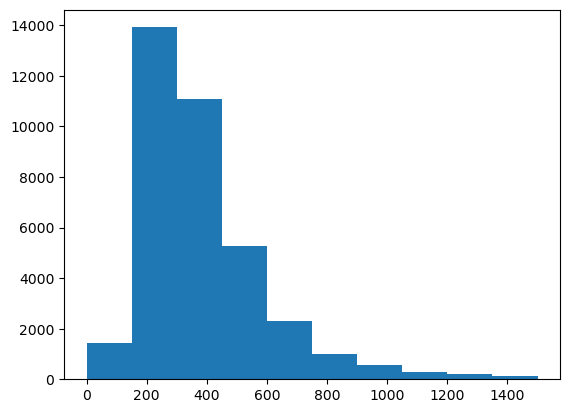
\includegraphics[width=0.6\textwidth]{tok_len_hist.png}
        \caption{Гистограмма распределения количества токенов в объектах тренировочного набора}
        \label{fig:tok_len_hist}
    \end{figure}
    \par Из рисунка \ref{fig:tok_len_hist} видно, что оптимальным количеством токенов для рассмотрения будет 1000, что в 5 раз больше привычного количества токенов у блока. Соответственно вычисление attention становится медленнее в 25 раз.
    \par В связи с неэффективностью стандартного attention слоя было решено использовать встроенный в PyTorch FalshAttention\cite{dao2022flashattentionfastmemoryefficientexact}. Таким образом удалось существенно увеличить скорость работы и уменьшить потребление памяти.
    \par После этих изменений модель смогла работать с большими последовательностями токенов.

    \subsubsection{Multcirop augmentation}
    \par Для обработки текста методом, аналогичным разбиению изображений на кропы, исходный текст сначала преобразуется в последовательность токенов. Затем эта последовательность делится на блоки случайного размера.
    \par Для улучшения качества семантической значимости блоков можно делить код, основываясь на символе переноса строки, так как оконченная строка программного кода, по сути своей, уже является логическим выражением.
    \par Развивая прошлую идею можно использовать инструменты для синтаксического анализа кода, чтобы разбивать текст на блоки, благодаря ветвям синтаксического дерева. Такой подход позволяет получать завершенные логические блоки.
    \par В конечной реализации было решено использовать разделение блоков по токенам, таким образом получится больше уникальных блоков в небольшом наборе данных, что значительно увеличит разнообразие в данных.
    \subsubsection{Аугментация данных}
    \par Аугментация текстовых данных является нетривиальной задачей, к которой есть несколько подходов.
    \begin{itemize}
        \item Синтаксические методы -- изменение структуры предложения с сохранением смысла. Основные способы: замена на синонимы, перестановка слов, добавление/удаление стоп слов.
        \item Семантические методы -- использование моделей для генерации новых вариантов текста. Основные способы: обратный перевод, генерация текста с помощью LLM, замена слов через предобученые \acrshort{mlm} модели.
        \item Методы основанные на шуме -- добавление шума для повышения устойчивости модели. Основные способы: случайные вставки/удаления слов, обмен местами соседних букв или слов, имитация ошибок клавиатуры.
    \end{itemize}
    \par В конкретном случае в связи с тем что данные являются кодом на языке C, синтаксические методы не подойдут из-за невозможности определения поведения методов и функций. Семантические методы не подходят из-за специфики данных. А методы на основе шума не подходят из-за того, что такие ошибки чаще всего отметаются спелчекермо из современных IDE.
    \par После определения необходимых аугментаций все остальные были удалены.
\end{document}
